\chapter{계량, 팽창, 그리고 첫 우주론}

앞선 강의의 끝에서 우리는 로런츠 불변 파동 방정식에 도달했고, 맥스웰 방정식을 시공간 형식으로 쓰려던 참이었습니다.
이제 중력으로 넘어가기 전에 청중의 질문 하나를 통해 유용한 주의점을 짚고 가겠습니다. 대칭성만으로 물리 이론의 어느 정도까지 결정할 수 있을까요?
답은 단호합니다. 상당히 많은 부분을 결정하지만, 전부는 아닙니다. 로런츠 불변성은 가능한 법칙을 강력하게 걸러 줍니다. 하지만 나머지 물리적 가정이나 실험을 대신하지는 못합니다.

\section{대칭성만으로 결정되지 않는 것}

\begin{classroomqa}
\audiencequestion{전기장과 자기장이 로런츠 변환 아래에서 함께 변환된다는 사실을 알고 있다면, 상대성 원리만으로 맥스웰 방정식이 따라 나오나요?}
\lecturerresponse{아닙니다. 상대성 원리는 방정식의 형태를 제약하지만, 방정식을 구성할 때는 선형성, 미분의 차수가 낮다는 점, 장이 변환하는 방식, 그리고 실험 정보도 사용합니다.
이러한 추가 요소가 없다면 로런츠 공변인 장 방정식은 여전히 무수히 많이 가능합니다.}
\end{classroomqa}

도입부에서 추가 가정 가운데 가장 중요한 것은 선형성입니다. \(A(x,t)\)가 선형 장 방정식의 해라면, 임의의 상수 \(\lambda\)에 대해 \(\lambda A(x,t)\)도 해입니다. \(A\)와 \(B\)가 해라면, \begin{equation}
  C(x,t)=A(x,t)+B(x,t).
  \label{eq:superposition}
\end{equation} 역시 해입니다.
이것이 중첩 원리입니다. 진공에서 전자기파 두 개가 서로 교차해도 각각 그대로 나아갈 수 있습니다. 물체가 충돌하듯 서로 직접 부딪히지는 않습니다. 각 파동이 전하를 움직이고 움직이는 전하가 복사를 방출하므로 하전 물질을 통해 간접적으로 상호작용할 수는 있지만, 진공 장 방정식 자체는 선형입니다.

\begin{figure}[H]
\centering
\includegraphics[width=0.64\textwidth]{lecture_08_figure_01.png}
\caption{중첩을 설명할 때 칠판에 그린 두 파동의 프로필. 두 파동의 합도 진공에서 허용되는 파동입니다.}
\lectureframe{00:05:30}
\end{figure}

조화 진동자를 보면 대수적인 구조가 분명해집니다. \begin{equation}
  m\ddot x=-kx.
  \label{eq:linear-oscillator}
\end{equation}라고 합시다.
\(x_1\)와 \(x_2\)가 \eqref{eq:linear-oscillator}를 만족하면, \begin{equation}
  m(\ddot x_1+\ddot x_2)
  =-k(x_1+x_2),
\end{equation}이므로 \(x_1+x_2\)도 해입니다. 그러나 비선형 항을 더해 \begin{equation}
  m\ddot x=-kx+p x^2,
  \label{eq:nonlinear-oscillator}
\end{equation}로 만들면 합은 더 이상 해가 아닙니다. \begin{equation}
  (x_1+x_2)^2=x_1^2+x_2^2+2x_1x_2.
\end{equation}에서 교차항 \(2x_1x_2\)이 나타나는데, 두 개별 방정식에는 이에 대응하는 항이 없습니다. 이제 두 운동은 서로 영향을 줍니다.

\begin{figure}[H]
\centering
\includegraphics[width=0.73\textwidth]{lecture_08_figure_02.png}
\caption{각 진동자의 방정식과 두 진동자의 합에 대한 방정식을 비교한 그림. 이차항에서 중첩을 깨뜨리는 추가 교차항이 드러납니다.}
\lectureframe{00:10:10}
\end{figure}

이 예는 우주론 논의 내내 유지할 방법론적 요점을 분명히 합니다. 대칭성은 어떤 양을 결합할 수 있는지, 어떤 방정식이 허용되는지를 알려 줍니다. 자연이 허용된 방정식 가운데 실제로 어떤 것을 따르는지는 동역학과 관측이 알려 줍니다.

\section{기하학으로서의 간격}

이제 전자기학을 떠나 일반 상대성 이론과 우주론으로 짧게 들어가 보겠습니다. 출발점은 서로 이웃한 사건 사이의 간격입니다. 한 사건의 좌표를 \(x^\mu\)로, 그 가까이에 있는 다른 사건의 좌표를 \(x^\mu+dx^\mu\)로 표시합시다. 관성 직교 좌표에서 \(c=1\)이고 \((+,-,-,-)\) 부호 규약을 쓰면,
\begin{equation}
  d\tau^2
  =dt^2-dx^2-dy^2-dz^2
  =dx^\mu dx_\mu
  =\eta_{\mu\nu}\,dx^\mu dx^\nu.
  \label{eq:minkowski-interval}
\end{equation}
불변인 것은 어느 한 좌표 차이가 아니라 \(d\tau^2\)입니다. 로런츠 변환은 이 이차 결합을 보존하면서 \(dt,dx,dy,dz\)를 바꿉니다. 따라서 특수 상대성 이론은 민코프스키 시공간의 기하학으로 이해할 수 있습니다.

\begin{figure}[H]
\centering
\includegraphics[width=0.72\textwidth]{lecture_08_figure_03.png}
\caption{성분 표기, 축약된 지표 표기, 계량 텐서 표기로 차례로 쓴 민코프스키 간격.}
\lectureframe{00:14:50}
\end{figure}

\eqref{eq:minkowski-interval}가 단순한 형태를 띠는지는 좌표에 달려 있습니다. 평면도 좌표를 적절하지 않게 잡으면 익숙하지 않은 계수가 나타날 수 있습니다. \(x\)는 센티미터로, \(y\)는 미터로 측정한다고 합시다. 물리적 변위에 대해서는 \begin{equation}
  ds^2=dx^2+\left(\frac{dy}{100}\right)^2
      =dx^2+10^{-4}dy^2.
  \label{eq:mixed-units}
\end{equation}입니다.
계수 \(10^{-4}\)에는 곡률에 관한 정보가 없습니다. 단지 단위를 서로 변환할 뿐입니다.

\begin{figure}[H]
\centering
\includegraphics[width=0.59\textwidth]{lecture_08_figure_04.png}
\caption{한 축은 센티미터, 다른 축은 미터로 표시한 평면. 서로 다른 계량 계수는 곡률이 아니라 단위를 나타냅니다.}
\lectureframe{00:20:10}
\end{figure}

비스듬한 좌표를 쓰면 혼합항이 생깁니다. 2차원에서 가장 일반적인 국소 이차 형식은 다음과 같이 쓸 수 있습니다.
\begin{align}
  ds^2
  &=a_{11}\,dx^2+a_{12}\,dx\,dy\notag\\
  &\quad+a_{21}\,dy\,dx+a_{22}\,dy^2,
  \qquad a_{12}=a_{21}.
  \label{eq:quadratic-form}
\end{align}
보통의 미분량은 교환 가능하므로 \(dx\,dy=dy\,dx\)입니다. 따라서 계수 배열에서 대칭인 부분만 기여합니다. 계수들을 행렬로 모으면 \begin{equation}
  g=
  \begin{pmatrix}
    a_{11} & a_{12}\\
    a_{21} & a_{22}
  \end{pmatrix}.
  \label{eq:metric-matrix}
\end{equation}입니다.
이 행렬이 \emph{계량}입니다. 계량은 좌표 차이를 물리적 간격으로 바꾸는 국소 규칙입니다.

\begin{figure}[H]
\centering
\includegraphics[width=0.71\textwidth]{lecture_08_figure_05.png}
\caption{이차 미분 형식과, 이 행렬을 계량으로 식별하는 순간의 대칭 \(2\times2\) 계수 행렬.}
\lectureframe{00:24:07}
\end{figure}

직교 격자든 비스듬한 격자든 균일하면 계수는 상수입니다. 좌표선이 휘거나 서로 가까워지거나 멀어지면, 바탕 표면이 평평하더라도 계수는 위치의 함수가 됩니다. 시공간의 일반적인 표기법은 다음과 같습니다.
\begin{equation}
  ds^2=g_{\mu\nu}(x)\,dx^\mu dx^\nu.
  \label{eq:general-metric}
\end{equation}

\begin{figure}[H]
\centering
\includegraphics[width=0.66\textwidth]{lecture_08_figure_06.png}
\caption{좌표 격자가 위치에 따라 달라지도록 허용했을 때의 일반적인 위치 의존 계량.}
\lectureframe{00:28:10}
\end{figure}

지정된 좌표계에서 \(g_{\mu\nu}\)를 알면 국소적인 거리, 시간, 각도가 정해지고, 그에 따라 기하학도 정해집니다. 역은 유일하지 않습니다. 하나의 기하학에 무수히 많은 좌표 기술이 대응하므로, 좌표 변환으로 서로 연결되는 계수 함수 배열도 무수히 많습니다.

\section{좌표의 복잡성과 내재적 곡률}

이제 복잡한 계량과 휘어진 공간을 구별해야 합니다. 종이를 늘리지 않은 채 원통 모양으로 말아 보세요. 방 안에서 보이는 모양은 달라지지만, 종이 위에서 재는 거리는 모두 그대로입니다. 종이에 갇혀 사는 생명체는 내재적인 측정만으로는 휘어짐을 알아낼 수 없습니다. 이는 외재적 휘어짐이지, 여기서 말하는 곡률이 아닙니다.

반구는 다릅니다. 늘이거나 찢거나 압축하지 않고서는 평평하게 펼칠 수 없습니다. 지구를 평면 지도로 나타내면 거리, 넓이, 각도 중 하나 이상이 왜곡되어야 합니다. 이 제약은 내재적이며, 주변 차원을 들여다보지 않아도 알아낼 수 있습니다.

극좌표는 반드시 살펴봐야 할 평평한 반례입니다. 평면에서 미소한 반지름 방향 변위의 길이는 \(dr\)이고, 반지름 \(r\)에서 각변위 \(d\theta\)의 길이는 \(r\,d\theta\)입니다. 따라서 \begin{equation}
  ds^2=dr^2+r^2d\theta^2,
  \qquad
  g_{\text{polar}}=
  \begin{pmatrix}
    1&0\\
    0&r^2
  \end{pmatrix}.
  \label{eq:polar-metric}
\end{equation}입니다.
계수 \(r^2\)은 평면 곳곳에서 달라지지만, 평면은 평평합니다. 변수 변환 \begin{equation}
  x=r\cos\theta,\qquad y=r\sin\theta
\end{equation}을 하면 상수 계량 \(ds^2=dx^2+dy^2\)으로 돌아옵니다.

\begin{figure}[H]
\centering
\includegraphics[width=0.70\textwidth]{lecture_08_figure_07.png}
\caption{극좌표 계량과 데카르트 계량으로의 복귀. 왼쪽의 위치 의존 행렬도 여전히 평평한 평면을 나타냅니다.}
\lectureframe{00:39:20}
\end{figure}

\begin{classroomqa}
\audiencequestion{극좌표에서 각도 방향 거리에 사인 함수가 들어가야 하나요?}
\lecturerresponse{평면에서는 그렇지 않습니다. 평면에서 호의 길이는 \(r\,d\theta\)입니다. 사인 함수는 구면에서 나타나는데, 위도선을 이루는 원의 반지름이 \(R\sin\theta\)이기 때문입니다.}
\end{classroomqa}

반지름이 \(R\)인 구를 생각합시다. \(\theta\)는 북극에서부터 잰 극각이고 \(\phi\)는 방위각이라고 합시다. 자오선을 따라 한 걸음 움직인 길이는 \(R\,d\theta\)입니다. 극각이 \(\theta\)일 때 위도선을 이루는 원의 반지름은 \(R\sin\theta\)이므로, 방위각 방향으로 한 걸음 움직인 길이는 \(R\sin\theta\,d\phi\)입니다. 국소적인 피타고라스 정리에 따라 \begin{align}
  ds^2
  &=R^2\left(d\theta^2+\sin^2\theta\,d\phi^2\right),
  \label{eq:sphere-metric}\\
  g_{\text{sphere}}=
  &\begin{pmatrix}
    R^2&0\\
    0&R^2\sin^2\theta
  \end{pmatrix}.
\end{align}입니다.

\begin{figure}[H]
\centering
\includegraphics[width=0.72\textwidth]{lecture_08_figure_08.png}
\caption{구와 그 각도 방향 선요소, 그리고 이에 대응하는 계량 행렬. \(\sin^2\theta\) 인자는 위도선을 이루는 원의 반지름이 줄어드는 것을 나타냅니다.}
\lectureframe{00:45:15}
\end{figure}

\begin{figure}[H]
\centering
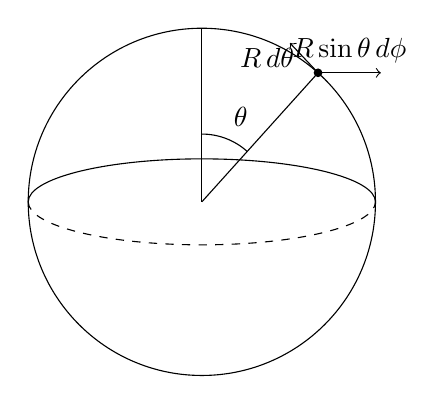
\begin{tikzpicture}[scale=1.05]
  \draw (0,0) circle (2.1);
  \draw[dashed] (-2.1,0) arc (180:360:2.1 and 0.52);
  \draw (2.1,0) arc (0:180:2.1 and 0.52);
  \coordinate (P) at (48:2.1);
  \fill (P) circle (1.5pt);
  \draw (0,0) -- (0,2.1);
  \draw (0,0) -- (P);
  \draw (0,0.82) arc (90:48:0.82);
  \node at (0.47,1.03) {\(\theta\)};
  \draw[->] (P) -- ++(-0.34,0.36)
    node[midway,left] {\(R\,d\theta\)};
  \draw[->] (P) -- ++(0.76,0)
    node[midway,above] {\(R\sin\theta\,d\phi\)};
\end{tikzpicture}
\caption{국소 미분 변을 구성해 \eqref{eq:sphere-metric}를 얻는 과정을 깔끔하게 다시 그린 그림.}
\end{figure}

전역적인 좌표 변환으로는 \eqref{eq:sphere-metric}를 상수 유클리드 행렬로 바꿀 수 없습니다. 2차원 관측자는 이를 내재적으로 알아낼 수 있습니다. 측지선으로 이루어진 충분히 큰 삼각형의 내각의 합이 \(180^\circ\)보다 큽니다. 따라서 유용한 판별 기준을 얻었습니다. 계수가 변한다고 해서 그 자체로 곡률이 있는 것은 아닙니다. 곡률이란 고려 중인 영역 전체에서 계량을 상수로 만드는 좌표를 찾을 수 없는 제약입니다.

\section{휘어진 시공간에서 우주론으로}

일반 상대성 이론에서는 시공간 자체가 내재적 곡률을 가질 수 있습니다. 위치 의존적인 \(g_{\mu\nu}\)도 극좌표의 경우처럼 좌표의 인공물일 수 있습니다. 그러나 실제로 휘어진 시공간에서는 어떤 좌표 변환으로도 그 변화를 전역적으로 없앨 수 없습니다.

\begin{figure}[H]
\centering
\includegraphics[width=0.70\textwidth]{lecture_08_figure_09.png}
\caption{특정 좌표계의 예에서 일반적인 시공간 선요소 \(ds^2=g_{\mu\nu}(x)dx^\mu dx^\nu\)로 넘어가는 과정.}
\lectureframe{00:48:40}
\end{figure}

아인슈타인 방정식의 전체 수학적 장치를 다루지는 않겠습니다. 대신 우주론에 적합한 기하학에만 주의를 기울이겠습니다. 충분히 큰 규모에서 공간은 균일하다고 보고, 기하학은 시간에 따라 변할 수 있다고 둡니다. 균일하다는 것은 한 위치도 다른 위치보다 특별하지 않다는 뜻입니다. 평평하다는 뜻은 아닙니다. 구면의 모든 점은 동등하지만 구면은 휘어져 있습니다. 또한 모든 규모에서 특징이 없다는 뜻도 아닙니다.

\begin{classroomqa}
\audiencequestion{은하들이 은하단, 판, 필라멘트를 이루는데도 우주는 어떻게 균질할 수 있습니까?}
\lecturerresponse{이 주장은 거친 평균을 취한 규모에 관한 것입니다. 별, 은하, 은하단은 매우 비균질합니다. 수억 광년 너비의 영역들을 비교하면, 그런 구조들을 평균했을 때 분포는 균일한 쪽으로 가까워집니다. 우주론적 원리는 논리적 필연이 아니라 관측에 근거한 잠정적 가설입니다. 우주 배경 복사의 방향에 따른 차이를 비롯해 충분히 큰 체계적 차이가 발견된다면 이 원리는 반증될 수 있습니다.}
\end{classroomqa}

이번 강의에서 두 번째로 세우는 대규모 가정은 공간이 평평하다는 것입니다. 우주 시간의 한 순간에 충분히 큰 삼각형은 유클리드 기하를 따르는 것처럼 보이며, 내각의 합은 \(180^\circ\)입니다. 이는 3차원 공간의 기하학에 대한 진술이지, 아직 4차원 시공간의 곡률에 대한 진술은 아닙니다.

\begin{classroomqa}
\audiencequestion{우주론적 거리에 떨어져 있는 점들에서는 동시성이 무엇을 뜻합니까? 그 점들에서 온 빛은 서로 다른 시각에 우리에게 도달하는데요.}
\lecturerresponse{먼 은하들 사이에 막대를 놓거나 그 은하들을 순간적으로 살펴볼 수는 없습니다. 우리는 신호를 나중에 받아 시공간 모형 안에서 그 신호를 방출한 사건들의 기하학적 관계를 재구성합니다. 이 절차는 간접적이지만, 천문학의 여러 기하학적 측정도 마찬가지입니다. 평탄하다는 것은 조사한 규모에서 재구성한 큰 삼각형들에 감지할 수 있는 각도 초과나 부족이 없다는 뜻입니다.}
\end{classroomqa}

\section{공동이동 좌표와 척도 인자}

은하의 대규모 흐름에 데카르트 격자를 그려 놓았다고 상상해 봅시다. 격자가 팽창해도 각 은하는 자기 좌표 표지를 그대로 유지합니다. 이 표지는 미터 단위의 거리가 아니라 위치를 가리키는 주소입니다. 시간에 따라 변하는 환산 인자가 좌표 간격을 물리적 거리로 바꾸어 줍니다.

\begin{figure}[H]
\centering
\begin{tikzpicture}[>=Latex,scale=0.86]
  \foreach \x in {0,0.65,1.3,1.95,2.6} {
    \draw[gray!65] (\x,0) -- (\x,2.2);
  }
  \foreach \y in {0,0.55,1.1,1.65,2.2} {
    \draw[gray!65] (0,\y) -- (2.6,\y);
  }
  \fill[blue!65!black] (0.65,0.55) circle (2pt);
  \fill[red!70!black] (1.95,1.65) circle (2pt);
  \node[below] at (1.3,-0.2) {comoving labels at \(t_1\)};
  \draw[->,very thick] (3.0,1.1) -- (4.0,1.1)
    node[midway,above] {\(a(t)\) grows};
  \foreach \x in {4.4,5.5,6.6,7.7,8.8} {
    \draw[gray!65] (\x,0) -- (\x,2.2);
  }
  \foreach \y in {0,0.55,1.1,1.65,2.2} {
    \draw[gray!65] (4.4,\y) -- (8.8,\y);
  }
  \fill[blue!65!black] (5.5,0.55) circle (2pt);
  \fill[red!70!black] (7.7,1.65) circle (2pt);
  \node[below] at (6.6,-0.2) {same labels at \(t_2\)};
\end{tikzpicture}
\caption{격자의 물리적 간격이 커져도 공동이동 주소는 고정되어 있습니다.}
\end{figure}

공간적 균일성을 만족하려면 같은 시각에 공간 어디서나 환산 인자가 같아야 합니다. 공간적 평탄성을 만족하려면 계량의 공간 부분을 데카르트 형식으로 쓸 수 있습니다. 그러면 선요소는 다음과 같습니다.
\begin{equation}
  d\tau^2
  =dt^2-a^2(t)\left(dx^2+dy^2+dz^2\right).
  \label{eq:flrw-flat}
\end{equation}
이는 공동이동 좌표로 쓴 공간적으로 평평하고 균일한 우주론적 계량입니다. \(x,y,z\)를 무차원으로 두고 \(a(t)\)에 길이 단위를 부여할 수 있습니다. 다른 규약에서는 좌표에 차원을 두고 \(a\)를 무차원으로 둘 수도 있습니다. 중요한 것은 두 양의 곱뿐입니다.

\begin{figure}[H]
\centering
\includegraphics[width=0.76\textwidth]{lecture_08_figure_10.png}
\caption{세 공간 방향 모두에 공통 인자 \(a^2(t)\)가 곱해지도록 칠판에 완성한 공간적으로 평평한 우주론적 계량.}
\lectureframe{01:03:15}
\end{figure}

\(a\)가 상수라면 \(x,y,z\)의 크기를 재조정해 흡수할 수 있고, \eqref{eq:flrw-flat}는 단위만 다른 보통의 민코프스키 시공간이 됩니다. 척도 인자가 시간에 따라 변한다는 점이 비자명한 요소입니다.

\begin{classroomqa}
\audiencequestion{좌표 격자가 팽창한다면, 왜 미터 자와 원자, 은하는 함께 팽창하지 않습니까?}
\lecturerresponse{계량은 우주적 흐름의 평균을 나타내며, 모든 결합계가 그 흐름을 따르도록 강제하는 힘을 뜻하지는 않습니다. 전자기력이 미터 자와 원자를 결합해 두고, 자체 중력이 은하를 결합해 둡니다. 작은 규모에서는 이런 결합 효과가 배경 팽창의 극히 약한 영향보다 큽니다. 가까운 은하들은 허블 흐름에서 벗어날 수도 있습니다. 안드로메다는 우리은하 쪽으로 끌려오고 있습니다. 은하의 결합을 자세히 연구해 보면 보이는 물질만으로는 충분하지 않다는 사실이 드러나며, 이는 암흑 물질을 뒷받침하는 논거 중 하나입니다.}
\end{classroomqa}

\begin{classroomqa}
\audiencequestion{척도 인자 자체가 은하들을 서로 밀어내는 힘이 아닌 이유는 무엇입니까?}
\lecturerresponse{현재의 규약에서 척도 인자는 길이 차원을 가지며, 힘의 차원을 갖지 않습니다. 위로 발사된 포탄을 생각해 보십시오. 발사된 뒤 포탄의 바깥쪽 운동은 관성 운동이며, 중력은 속도를 줄이거나 포탄을 되돌아오게 함으로써 그 운동을 바꿉니다. 마찬가지로 팽창은 운동 상태입니다. 역학에서 물어야 할 것은 중력과 다른 원천들이 \(\dot a\)와 \(\ddot a\)를 어떻게 바꾸는가이지, \(a\)가 계속 운동하도록 어떤 힘이 필요한가가 아닙니다.}
\end{classroomqa}

예전에는 인력이 작용하는 중력이 팽창을 감속시킬 것이라고 예상했습니다. 이 강의가 진행될 무렵에는 천문학적 증거를 통해 최근의 팽창이 오히려 가속되고 있음이 밝혀졌습니다. 이는 전체 동역학에 보통의 인력을 받는 물질 이상의 요소가 포함된다는 뜻입니다. 기하학적 토대를 확실히 다질 때까지 이 문제는 미뤄 두겠습니다.

\section{허블 법칙}

고정된 좌표 간격 \(\Delta x\)만큼 떨어진 공동이동 은하 두 개를 생각합시다. 같은 우주 시간에서 두 은하 사이의 물리적 거리는 \begin{equation}
  D(t)=a(t)\,\Delta x.
  \label{eq:physical-distance}
\end{equation}입니다.
공동이동 좌표 표지를 고정한 채 미분하면 \begin{align}
  V(t)
    &=\dot D(t)
      =\dot a(t)\,\Delta x \nonumber\\
    &=\frac{\dot a(t)}{a(t)}D(t).
  \label{eq:hubble-derivation}
\end{align}입니다.
\begin{equation}
  H(t)=\frac{\dot a(t)}{a(t)}.
  \label{eq:hubble-parameter}
\end{equation}로 정의하면 \begin{equation}
  V(t)=H(t)D(t).
  \label{eq:hubble-law}
\end{equation}입니다.
한 우주 시각에는 같은 \(H(t)\)가 공간 어디서나 적용되어야 합니다. 그렇지 않으면 공간이 균일하지 않을 것입니다. 공동이동 격자의 모든 간격이 같은 분율만큼 늘어나므로 후퇴 속도는 거리에 비례합니다.

\begin{figure}[H]
\centering
\includegraphics[width=0.73\textwidth]{lecture_08_figure_11.png}
\caption{물리적 거리 \(D=a\Delta x\)와 이를 시간에 대해 미분해 \(V=(\dot a/a)D\)에 이르는 과정.}
\lectureframe{01:16:45}
\end{figure}

\begin{classroomqa}
\audiencequestion{먼 은하에 대해서는 허블 매개변수를 현재 시각에 평가해야 합니까, 아니면 관측된 빛이 방출된 시각에 평가해야 합니까?}
\lecturerresponse{기술하려는 시점의 값을 써야 합니다. 먼 은하에서 온 빛은 팽창의 과거 값을 알려 줍니다. 제대로 분석하려면 \(H\)의 시간에 따른 변화를 고려해야 합니다. 오늘날의 값을 모든 곳에 대입하는 것은 국소적인 근사일 뿐입니다.}
\end{classroomqa}

\begin{classroomqa}
\audiencequestion{\(D=a\Delta x\)에서 단위는 어디에 들어 있습니까?}
\lecturerresponse{편리한 방법은 공변 좌표 \(\Delta x\)를 무차원으로 두고 \(a\)가 길이 단위를 갖도록 하는 것입니다. 반대로 단위를 정할 수도 있습니다. 어느 쪽으로 정하든 \(H=\dot a/a\)는 역시간 차원을 가집니다.}
\end{classroomqa}

\section{팽창 좌표계에서의 빛}

빛은 영 경로를 따릅니다. 그런 경로를 따라 고유 시간 간격은 영이 됩니다.
\begin{equation}
  d\tau^2=0.
\end{equation}

\begin{classroomqa}
\audiencequestion{빛에 대해서는 왜 간격이 영인가요?}
\lecturerresponse{상대론에서 빛살의 기하학을 정의하는 성질이 바로 그것입니다. 국소적으로 자유 낙하하는 모든 관측자는 빛의 속력을 \(c=1\)라고 측정하므로, 국소적으로 \(dt^2=d\ell^2\)가 성립하고 시공간 간격은 영이 됩니다. 그렇다고 빛을 받는 관측자에게 좌표 시간이 흐르지 않는다는 뜻은 아닙니다.}
\end{classroomqa}

\(x\) 방향으로만 움직이는 광선에 대해서는 \begin{equation}
  0=dt^2-a^2(t)\,dx^2.
\end{equation}입니다.
\(x\)가 증가하는 방향으로 움직이는 광선을 택하면 \begin{equation}
  dt=a(t)\,dx,
  \qquad
  dx=\frac{dt}{a(t)},
  \qquad
  \frac{dx}{dt}=\frac{1}{a(t)}.
  \label{eq:null-ray}
\end{equation}입니다.

\begin{figure}[H]
\centering
\includegraphics[width=0.64\textwidth]{lecture_08_figure_12.png}
\caption{팽창 계량의 영 조건과 그에 따라 얻는 공동이동 좌표에서의 광선 방정식 \(dx=dt/a(t)\).}
\lectureframe{01:23:45}
\end{figure}

척도 인자가 커질수록 좌표 속도 \(dx/dt\)는 감소합니다. 그렇다고 빛이 국소적으로 느려진다는 뜻은 아닙니다. 공동이동 좌표 거리 한 단위가 점점 더 큰 물리적 거리에 해당하므로 수치로 나타낸 좌표 속도는 달라지지만, 모든 국소 측정값은 여전히 \(c=1\)입니다.

\section{시간 의존성이 중요한 이유}

이제 핵심 기하학적 질문을 피할 수 없습니다. \(a(t)\)는 어떻게 변할까요? 위치를 어느 한 순간에만 알고 있는 발사체를 비유로 들어 보겠습니다. 미래 궤적을 알려면 운동 방정식이 필요합니다. 우주론에서는 중력 동역학이 \(a(t)\)에 대한 방정식을 제공할 것입니다.

\begin{classroomqa}
\audiencequestion{\(a(t)\)가 변하는지를, 전자의 전하 같은 다른 물리량이 시간에 따라 변하는지를 묻는 것보다 더 중요하게 여기는 이유는 무엇입니까?}
\lecturerresponse{논리적 위계는 없습니다. 전자의 전하가 변한다는 측정 결과가 나오면 대단히 중요한 발견일 것입니다. 우리는 \(a(t)\)에 주목합니다. 관측 결과 우주적 거리들은 이미 변하고 있지만 전자의 전하는 일정한 것으로 보이기 때문입니다. 기하학적으로는 일정한 \(a\)를 공간 단위의 변경으로 없앨 수 있으며, 그렇게 해도 평탄한 시공간은 그대로입니다. 시간에 따라 변하는 \(a\)는 그런 방식으로 없앨 수 없습니다.}
\end{classroomqa}

먼 은하의 후퇴를 측정하기에 앞서, 무엇을 측정하는지 말해 줄 기하학적 틀이 필요합니다. 가장 거칠게 보자면, 광도가 알려진 천체는 빛이 더 넓은 면적에 퍼지기 때문에 거리가 멀수록 어둡게 보입니다. 또한 알려진 원자 스펙트럼선의 이동으로 적색편이를 구해 후퇴의 지표로 삼습니다. 허블은 거리 추정치와 적색편이를 결합해 비례 관계 \eqref{eq:hubble-law}를 밝혀냈지만, 초기의 계수값은 상당히 틀렸습니다. 현대의 거리 사다리와 상대론적 빛 전파 계산은 훨씬 정교하지만, 개념적으로는 여전히 거리와 적색편이라는 두 요소를 함께 사용합니다.

\section{허블 시간과 우주 나이의 추정}

허블 법칙에는 간단한 추정법이 숨어 있습니다. 은하의 현재 후퇴 속도를 고정해 두고 그 운동을 일정한 속도로 거슬러 가 봅시다. 현재 거리를 좁히는 데 걸리는 시간은 \begin{equation}
  t=\frac{D}{V}.
\end{equation}입니다.
\(V=HD\)를 사용하면 \begin{equation}
  t=\frac{D}{HD}=\frac{1}{H}.
  \label{eq:hubble-time}
\end{equation}입니다.
거리가 약분되므로 공동이동 은하의 어느 쌍을 택해도 대략 같은 시간이 나옵니다. 여기서 서스킨드는 말로 하기 쉬운 실수를 짚어 바로잡습니다. 가정하는 것은 \(H\)가 일정하게 유지된다는 점이 아닙니다. 특정한 후퇴 속도가 일정하다고 보고 과거로 외삽하는 것입니다.

\begin{figure}[H]
\centering
\includegraphics[width=0.66\textwidth]{lecture_08_figure_13.png}
\caption{후퇴 속도를 과거로 외삽할 때 거리가 약분되는 허블 시간 추정 \(H^{-1}=D/(HD)=D/V\).}
\lectureframe{01:33:45}
\end{figure}

따라서 허블 매개변수의 역수는 시간 척도이지, 자동으로 우주의 정확한 나이가 되는 것은 아닙니다. 순수하게 감속하는 물질 지배 우주를 가정하고 현재 속도를 거꾸로 적용하면, 중력에 의해 은하들이 서로 끌려옵니다. 은하들은 등속도 운동일 때보다 더 빨리 만나므로 현재의 \(H^{-1}\)는 우주의 나이를 실제보다 크게 추정합니다. 강의에서는 허블 시간과 가깝지만 같지는 않은, 약 \(13.5\)억 년의 보정된 나이를 제시합니다.

\begin{classroomqa}
\audiencequestion{우리 은하 안에서는 허블 팽창이 없다면, 모든 은하의 운동을 거꾸로 돌려 은하들이 한데 모이게 한다는 말은 무슨 뜻입니까?}
\lecturerresponse{균질한 기술로는 결합된 구조의 실제 역사를 더는 묘사할 수 없는 시점에 이르게 됩니다. 시간의 정방향으로는 작은 요동이 중력에 의해 커져 은하와 은하단을 형성합니다. 영화를 문자 그대로 거꾸로 재생하려면 모든 미시적 운동이 반전되고 엔트로피가 감소해야 합니다. 평균적인 허블 흐름만 역전한다고 해서 구조 형성이 되돌려지지는 않습니다. 과거로의 외삽은 우주론적 규모에서 얻는 근사치이지, 모든 별이 지나온 경로를 되짚는 영화가 아닙니다.}
\end{classroomqa}

\begin{classroomqa}
\audiencequestion{은하 사이의 거리가 늘어나는 것과 자의 길이가 줄어드는 것을 실험으로 구별할 수 있습니까?}
\lecturerresponse{관측 가능한 것은 무차원 비율뿐입니다. 측정되는 것은 은하 사이의 거리를 원자 길이 또는 실험실 길이의 표준으로 나눈 비율이 증가한다는 사실입니다. 관례적으로 원자 물리와 분자 물리의 매개변수는 고정해 두고 우주가 팽창한다고 말합니다. 은하 사이의 거리를 표준으로 삼고 원자와 양성자, 미터 자의 길이가 줄어든다고 서술할 수도 있습니다. 그 비율에 관한 물리는 달라지지 않습니다.}
\end{classroomqa}

원자는 막대의 재료이고 크기는 일정해 보이는 매개변수에 의해 정해지므로 이런 규약은 자연스럽습니다. 미터는 궁극적으로 미시적 길이를 여러 번 이어 놓은 큰 값입니다. 이 미시적 표준을 고정해 두면 익숙한 표현대로 \(a(t)\)가 커집니다.

\begin{classroomqa}
\audiencequestion{\eqref{eq:flrw-flat}은 공간적 균질성과 평탄성을 만족하는 유일한 계량인가요?}
\lecturerresponse{좌표 변환에 따른 차이를 제외하면 유일합니다. 정확히 말하면, 그런 가정 아래 적절한 우주 시간과 공변 공간 좌표를 택했을 때 계량을 이 형태로 나타낼 수 있다는 뜻입니다. 다른 좌표계를 쓰면 같은 시공간도 상당히 다르게 보일 수 있습니다.}
\end{classroomqa}

\begin{classroomqa}
\audiencequestion{뒤로 계산한 은하 사이의 거리가 0에 이르면 허블 법칙으로 계산한 속도도 0이 됩니다. 그러면 은하들이 만나는 일을 막지 않습니까?}
\lecturerresponse{아닙니다. 오늘 추론한 \(H\)를 과거 내내 고정된 값으로 두지 않습니다. 일반적인 팽창 해에서는 과거에 \(H(t)\)가 훨씬 컸습니다. \(H_0^{-1}\)라는 추정치는 오늘날의 속도를 일정하게 연장해 규모를 얻을 뿐입니다. 실제 \(a(t)\)와 \(H(t)\), 속도는 역학으로 구해야 합니다.}
\end{classroomqa}

\section{뉴턴의 껍질 정리와 우주론적 동역학}

동역학을 알아내기 위해 은하들을 균일한 매질로 퍼뜨려 봅시다. 한 은하를 원점으로, 다른 은하의 공동이동 좌표 표지를 \(x\)로 정합시다. 이렇게 정하는 데 물리적 특권은 없습니다. 균일성에 따라 최종 방정식은 어느 은하를 기준으로 하든 같아야 합니다. 두 번째 은하의 물리적 반지름은 \begin{equation}
  R(t)=a(t)x.
  \label{eq:radius-ax}
\end{equation}입니다.

처음에는 그 은하의 중력을 구하려면 광대한 우주에 있는 모든 은하의 인력을 합산해야 할 것처럼 보입니다. 뉴턴의 껍질 정리가 문제를 단순하게 만듭니다.

\begin{proposition}[Newton's shell theorem]역제곱 힘과 구대칭 질량 분포의 경우, 시험점이 놓인 구 바깥의 물질은 순힘에 기여하지 않습니다. 구 안에 든 물질은 모두 구의 중심에 모여 있는 것처럼 시험점에 작용합니다.\end{proposition}

\begin{figure}[H]
\centering
\includegraphics[width=0.70\textwidth]{lecture_08_figure_14.png}
\caption{균일하게 분포한 은하들, 공동이동 좌표 표지 \(x\)에 있는 시험 은하, 그리고 그 안에 든 질량만이 시험 은하의 반지름 방향 운동을 결정하는 구.}
\lectureframe{01:50:05}
\end{figure}

\begin{figure}[H]
\centering
\begin{tikzpicture}[scale=0.94,>=Latex]
  \draw[gray!65] (0,0) circle (2.35);
  \foreach \p in {
    (-1.5,0.8),(-1.2,-0.8),(-0.8,1.5),(-0.6,0.35),(-0.3,-1.45),
    (0.15,1.05),(0.35,-0.55),(0.7,1.65),(0.9,0.45),(1.25,-0.9),
    (1.65,0.95),(-1.75,-0.2),(1.8,-0.15)} {
    \fill[black!55] \p circle (1.15pt);
  }
  \fill[blue!65!black] (0,0) circle (2pt)
    node[below left] {chosen origin};
  \fill[red!70!black] (2.35,0) circle (2.2pt)
    node[right] {test galaxy};
  \draw[->,thick] (0,0) -- (2.32,0)
    node[midway,above] {\(R=a(t)x\)};
  \draw[<->] (-2.35,-2.55) -- (2.35,-2.55)
    node[midway,below=4pt] {only the enclosed mass contributes};
\end{tikzpicture}
\caption{껍질 정리의 설정을 깔끔하게 다시 그린 그림. 원점은 편의를 위한 선택이지 우주의 중심이 아닙니다.}
\end{figure}

그리하여 우주론의 다체 문제는 익숙한 일체 문제로 바뀌었습니다. 현재 구 안에 포함된 질량의 인력을 받으며 반지름 방향으로 움직이는 발사체 문제입니다. 뉴턴 방정식으로 \(R=a x\)가, 따라서 \(a(t)\)가 어떻게 가속하는지 정할 수 있습니다. 강의에서는 이 계산을 수행하기 전에 의도적으로 멈춥니다. 다음 시간에는 기하학적 설정에 답을 슬며시 끼워 넣지 않고, 가장 단순한 물질 지배 우주론을 유도하겠습니다.

\section{마지막 질문: 빛, 빅뱅, 곡률}

정식 강의는 끝났지만, 마지막 질문들은 몇 가지 오해를 부르는 그림을 드러냅니다. 이는 부록이 아니라 물리학의 일부입니다.

\begin{classroomqa}
\audiencequestion{아주 먼 천체에서 온 빛이 우주가 훨씬 작았을 때 방출되었다면, 왜 지금은 그 천체가 아주 멀리 있는 것처럼 보일까요? 초기 우주가 조밀했다면, 왜 우주의 전부를 관측할 수는 없을까요?}
\lecturerresponse{팽창하는 좌표계에서 영선 방정식을 풀어야 합니다. \(a(t)\)가 매우 작을 때는 \(dx/dt=1/a(t)\)가 매우 큽니다. 빛은 국소적으로 \(c=1\)의 속도로 움직이면서 큰 공변 구간을 가로지릅니다. \(a(t)\)가 커질수록 공변 좌표 속도는 감소합니다. 정확한 방출 지점과 관측 가능한 영역의 크기는 \(a(t)\)의 전체 역사에 달려 있으므로, 구체적인 우주론을 풀 때까지 수치 답은 미뤄 둡니다.}
\end{classroomqa}

\begin{figure}[H]
\centering
\includegraphics[width=0.72\textwidth]{lecture_08_figure_15.png}
\caption{\((x,t)\) 평면에서의 광선: \(a(t)\)가 작을 때는 공변 좌표에서 거의 수평이며, 스케일 인자가 커질수록 점차 더 가파르게 기울어진다.}
\lectureframe{01:56:20}
\end{figure}

\eqref{eq:null-ray}를 적분하면 미뤄 둔 계산이 명시적으로 드러납니다.
\begin{equation}
  \Delta x
  =\int_{t_{\mathrm e}}^{t_0}\frac{dt}{a(t)}.
  \label{eq:comoving-light-distance}
\end{equation}
\(t_{\mathrm e}\)가 시작점에 가까워질 때 적분이 임의로 큰 공변 거리에 이르는지는 \(a(t)\)의 초기 시간 형태에 달려 있습니다.\editorialnote{식 \eqref{eq:comoving-light-distance}은 칠판에 적은 방정식 \(dx=dt/a(t)\)을 적분한 형태입니다. 특정 스케일 인자를 택하지 않은 채 다음 시간에 다루기로 한 계산을 명시적으로 보여 줍니다.}

\begin{figure}[H]
\centering
\begin{tikzpicture}[scale=0.92,>=Latex]
  \draw[->] (0,0) -- (6.4,0) node[right] {\(x\)};
  \draw[->] (0,0) -- (0,4.6) node[above] {\(t\)};
  \draw[thick,blue!65!black]
    plot[smooth] coordinates {(0,0.18) (1.65,0.42) (2.65,1.05)
      (3.35,2.05) (3.85,3.25) (4.05,4.25)};
  \fill[red!70!black] (4.05,4.25) circle (2pt)
    node[right] {reception today};
  \draw[dashed] (4.05,0) -- (4.05,4.25);
  \node[align=left] at (1.65,3.25)
    {\(\displaystyle \frac{dx}{dt}=\frac1{a(t)}\)\\
     large when \(a\) is small};
\end{tikzpicture}
\caption{공변 좌표로 나타낸 광선 구성을 깔끔하게 정리한 그림. 기울기가 변하는 것은 좌표 효과이지, 빛의 국소 속도가 변하는 것이 아니다.}
\end{figure}

\begin{classroomqa}
\audiencequestion{빅뱅 때 물질이 한 점에서 튀어나와 지금은 팽창하는 껍질이나 고리 위에 놓여 있어야 하나요?}
\lecturerresponse{아닙니다. 이 모형은 균일하고 극도로 밀도가 높은 공간에서 시작합니다. 모든 큰 규모의 거리가 늘어나는 것이지, 물질이 선호되는 중심에서 기존의 빈 공간을 가로질러 발사되는 것은 아닙니다. 표면 전체에 점들이 균일하게 찍힌 풍선은 유용한 2차원 비유입니다. 풍선이 팽창하면 점들 사이의 거리는 모두 늘어나지만 표면에는 점들이 계속 균일하게 분포합니다. 우주는 모든 양의 시간에서 무한할 수도 있습니다. 팽창한다고 해서 우주가 다른 무언가 안에 놓인 유한한 공으로 시작했다는 뜻은 아닙니다.}
\end{classroomqa}

\begin{classroomqa}
\audiencequestion{팽창하는 동안 중력 자체가 더 약하거나 강했나요?}
\lecturerresponse{이 논의에서는 뉴턴 상수 \(G\)를 고정된 값으로 둡니다. 그럼에도 거리와 내부에 포함된 밀도가 변하므로 힘은 달라집니다. 더 이른 시기에는 같은 공변 은하가 물리적으로 더 가까웠고 균일한 물질의 밀도도 더 높았으므로 중력에 의한 감속이 더 컸습니다. 바로 이 점을 정량화하는 것이 구각 정리 계산의 목적입니다.}
\end{classroomqa}

마지막으로 공간의 곡률과 팽창을 혼동해서는 안 됩니다. 지구의 반지름에 비해 크기가 아주 작은 지표면 일부는 평평해 보입니다. 충분히 큰 삼각형을 측정하면 각도의 초과량을 검출하거나 곡률 반지름의 하한을 정할 수 있습니다. 천문학에서는 엄청나게 큰 삼각형으로 이와 유사한 실험을 합니다. 2006 강의에서 사용한 관측 용어로 말하면, 관측 가능한 영역 전체에서 곡률이 검출되지 않았으므로 곡률 반지름은 그 영역보다 훨씬 커야 했습니다. 그렇다고 우주가 정확히 평평하다는 뜻은 아닙니다. 관측 가능한 부분이 얼마나 휘어 있을 수 있는지를 제한한다는 뜻입니다.

구의 내재 곡률은 \(R^{-2}\)에 따라 스케일링된다. 따라서 구가 커질수록 국소적으로 더 평평해진다. 마찬가지로 균질한 우주의 공간 곡률이 영이 아니라면, 팽창에 따라 곡률 반지름이 커지고 크기가 고정된 국소 영역에서 보이는 곡률은 작아진다.
\editorialnote{\(R^{-2}\)에 따른 스케일링은 구가 커질수록 곡률의 수치가 감소한다는 강의의 설명을 표준적인 정량식으로 나타낸 것이다.}

\begin{classroomqa}
\audiencequestion{공간이 휘어 있다면 우주의 한 부분은 수축하고 다른 부분은 팽창해야 하나요?}
\lecturerresponse{아닙니다. 양수, 0, 음수의 공간 곡률은 각 우주 시간 단면의 기하를 나타냅니다. 팽창과 수축은 \(a(t)\)의 변화로 결정됩니다. 곡률이 있는 우주도 팽창할 수 있고, 평평한 우주도 수축할 수 있습니다. 위로 움직이는 발사체가 다시 떨어질 수 있듯이 팽창이 나중에 역전될 수도 있지만, 곡률 자체에 동시 수축이 내포된 것은 아닙니다. 동역학에서 따져야 할 것은 바깥쪽 운동이 내부 질량의 인력을 벗어나는지, 되돌아오는지, 아니면 임계 경계에 놓이는지입니다.}
\end{classroomqa}

탈출 속도와의 비교는 이 강의에서 칠판에 적어 다룬 마지막 핵심 개념입니다. 기하를 통해 계량, 허블 법칙, 광선 방정식을 얻었습니다. 뉴턴의 정리로 동역학은 한 구 안에 든 질량만으로 다룰 수 있게 되었습니다. 다음 강의는 바로 여기서 시작해야 합니다. \(a(t)\)을 결정하는 방정식과 팽창이 탈출하는지, 다시 수축하는지, 아니면 아슬아슬한 경계에 놓이는지를 묻는 문제를 다룹니다.
